\section{Motivation}

\citet{wals-9} claimed that the velar nasal  /ŋ/ is exceptional in its phonotactic distribution: virtually all languages that have phonemic /ŋ/ allow it in the final position, while over one-third of those languages prohibit it in the initial position. In fact, of 20 chapters concerning phonology in \citet{wals}, \citeauthor{wals-9}'s The Velar Nasal is the only chapter that deals with only a single segment. This creates an impression that the distributional asymmetry of /ŋ/ is an exception amongst the consonants of the languages of the world. However, a recent article on the distribution of rhotics also reported a similar asymmetry: in 39\% of the languages in the survey, word-initial rhotics are either completely absent or only appear in a low proportion of the lexicon \citep{labrune2021word}. This calls for a question: what about other consonants? Intuitively, some consonants are expected to also have such asymmetry, for example it should be rare to see /h/in the final position, while some others, like /m/ should be very likely to have a symmetric distribution. Unfortunately, I am unable to find any database that contains such information about the distribution of segments. Thus, this thesis is an attempt to build a small database of consonantal distributions of 20 languages to investigate the degrees of asymmetry of their consonants.

\section{Literature Review}

\subsection{The Velar Nasal}

\citet{wals-9} surveyed a total of 469 languages and divided them into three categories: no velar nasal (e.g. French), initial velar nasal (Cantonese), and no initial velar nasal (e.g. English). This categorization seems to imply that languages in the ``initial velar nasal'' category also allow velar nasal in the final position (because there is no ``no final velar nasal'' category). However, in further discussion, the author revelled that this is not true. Some languages only have the velar nasal in the initial position but not final, but there are two reasons for this. The first one is that it is a genuine asymmetry of this one consonant, like in Nenets. The other case is because the language does not allow any coda at all, like in Fijan. This is an important point to consider, since they are two different restrictions. Taking an OT constraints analogy, one is \textsc{NoCoda} constraint and the other is \textsc{*Coda-ŋ}. Should such distinction appear in the database for this thesis, they ought to be coded differently.

\subsection{Word-Initial Rhotic Avoidance}

\citet{labrune2021word} examined a phenomenon called ``Word-initial rhotic avoidance'' (WIRA) in a language sample size of 200. The list of languages used is obtained from the 200-language sample recommended in \citet{wals}. All four terms in the name need clarification to better understand this work. ``Word'' is a widely used term but lacks of a definite definition (see discussion in, for example, \citet{martin2017indeterminacy}). In \citet{labrune2021word}, the author adopted a hybrid classification system: if in a language, clitics or affixes allow word-initial rhotics but the full lexical words do not, then ``word'' means ``full lexeme'' (and thus such language will be classified as exhibiting WIRA). When no morphological unit accepts word-initial rhotics, ``word'' will be understood as ``morph'' or ``stem''. ``Initial'' here means the first segment of a word at the phonemic level, and not necessarily at the phonetic level, and so the author divided  WIRA into (phon)emic-WIRA and (phon)etic-WIRA. Etic-WIRA is further divided into two subtypes: (a) a phonemic rhotic phonetically realized as non-rhotic in word-initial position, and (b) a phonemic non-rhotic phonetically realized as rhotic in word-internal position (e.g. flapping in American English).``Rhotic'' is defined in the paper as liquids minus laterals. The full list is given in Figure \ref{fig:rhotics}. The uvular rhotics are termed conditional, this means that they will only be considered rhotic if no core rhotics exist in the language and they do not pattern with non-sonorant segments.

\begin{figure}[h]
    \centering
    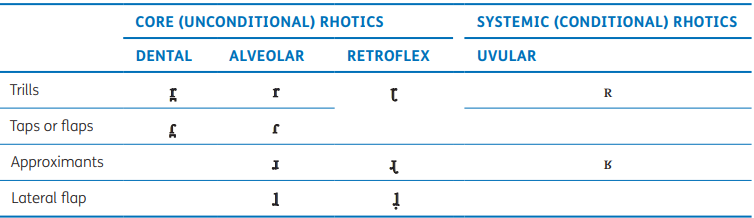
\includegraphics[scale=0.7]{rhotics.png}
    \caption{Rhotics list \citep[p.~4]{labrune2021word}}
    \label{fig:rhotics}
\end{figure}

``Avoidance'' is used instead of ``prohibition'' because, according to the author, the acceptance of rhotics in a language cannot always be answered with yes or no but is a matter of degree. An example given in the paper is that in a corpus of Maninka with over 28.000 tokens, rhotics appear 1564 times in total, but only 16 times in the initial position. The result of the paper is that 78 languages exhibit emic-WIRA and 30 languages exhibit etic-WIRA (nine of those also exhibit emic-WIRA). Since I will not investigate corpus in this thesis due to time restriction (and frequency data may not be mentioned in the descriptive grammar), the ``avoidance'' part is irrelevant to me. I will also not use the class of rhotics, or any other grouping, but just use the phoneme as the unit of investigation. The -emic and -etic distinction is relevant and will be further discuss in the methodology. 

\subsection{Language Sampling and WALS Sample List}

According to \citet{velupillai2012introduction}, there are three types of sampling used typological studies: probability sampling, variety sampling, and convenience sampling. Probability sampling aims to be statistically representative, and thus tries to achieve genealogical and areal balance in the sample. Variety sampling aims to include as much variations as possible, and thus may pay less attention to the genealogical or areal balance. Convenience sampling is, as its name, the sample that the researcher is able to access, though one can still try to be as diverse and representative as possible within it.

\par 
The World Atlas of Language Structures (WALS), while allowing the author of each chapter to choose the language sample they wish, provides a 100-language sample and a 200-language sample (built up on the 100-language sample) recommended to be included in every chapter \citep{wals-s1}. The 100 and 200 languages lists are constructed to maximize the diversity and to be representative of languages of the world, while also concern with the availability of descriptive data on the languages. The languages of the 100-language sample are more well-known and have more detailed description with better availability \citep{wals-s1}. Thus, the 100-language sample will be the starting point for constructing the 20-language sample in this thesis using semi-convenience sampling (more will be explained in the methodology).  

\subsection{Property-Driven Phonological Typology}

\citet{hyman2009not} claimed that there are two ways of doing typology: one focuses on classifying languages into ``types'', e.g. tone language and pitch-accent language, the other focuses on specific properties of the language. The paper is also a criticism on language classification and advocates for focusing on properties instead (i.e. property-driven typology). In this thesis, I will not attempt language classification, that is, I will not put languages into type like ``/\tipa{N}/ symmetric language'' or ``more symmetric language'' (based on the number of consonants that are symmetric in the language). I will only focus on the properties of each consonant in each language, the interest here are the segments themselves and not the languages that contain them. 

\par
Arguably, with this focus on the segment, it could be better to sample the segments and not the languages, i.e. investigate the distribution of 20 segments in all languages instead of all segments in 20 languages. However, the dimensions for segment sampling would be too large. For example, the ideal database for choosing 20 segments to investigate would be PHOIBLE \citep{phoible}, but for each segment their presence would be counted in 3020 inventories of 2186 distinct languages. Within the scope of this thesis, that number would be impossible to work with, and so I need to choose a more viable approach of sampling based on language.  